\documentclass[12pt]{article}
\usepackage[left=16mm,right=16mm,top=20mm,bottom=25mm,nohead]{geometry}

% ===== Language, font, endcoding =====
\usepackage[T1]{fontenc}
\usepackage[polish]{babel}
\usepackage[utf8]{inputenc}
\usepackage{lmodern}
\usepackage{lingmacros}
\usepackage{polski}
\selectlanguage{polish}

% ===== Math =====
\usepackage{mathtools}
\usepackage{mathrsfs}
\usepackage{amsfonts, amsmath, amssymb, amsopn, amsthm}
\usepackage{latexsym}

% ===== Other =====
\usepackage{tree-dvips}
\usepackage{xparse}
\usepackage{physics}
\usepackage{pgfplots}
\usepackage{pgfplotstable}
\pgfplotsset{compat=1.5}
\usepackage{graphicx}
% \usepackage{bookmark}
\usepackage{enumitem}

% ===== Custom figure caption =====
\usepackage{caption}
\DeclareCaptionFormat{myformat}{\small{#1#2#3}}
\DeclareCaptionLabelSeparator{mysep}{:\space}

\captionsetup[figure]{name={Ilustracja},labelsep=mysep, format=myformat}


% ===== Custom math operators =====
\DeclareMathOperator{\log10}{lg}
\renewcommand{\lg}[1]{\log10\left( #1 \right)}
\newcommand{\Ltr}[1]{\ensuremath{\mathscr{L}\left\lbrace #1 \right\rbrace}}
\newcommand{\Linv}[1]{\ensuremath{\mathscr{L}^{-1}\left\lbrace #1 \right\rbrace}}
\newcommand{\Ztr}[1]{\ensuremath{\mathscr{Z}\left\lbrace #1 \right\rbrace}}
\newcommand{\Zinv}[1]{\ensuremath{\mathscr{Z}^{-1}\left\lbrace #1 \right\rbrace}}
\newcommand{\Lim}[1]{\raisebox{0.5ex}{\scalebox{1}{$\displaystyle \lim_{#1}\;$}}}
\newcommand{\R}{\mathbb{R}}



% ===== Array / Matrix size =====
\renewcommand*{\arraystretch}{1.15}

% ===== Custom colors =====
\usepackage{xcolor}
\definecolor{goldenrod}{RGB}{218,165,32}
\definecolor{royalblue}{RGB}{65,105,225}
\definecolor{slategrey}{RGB}{112,128,144}

\definecolor{codegreen}{rgb}{0,0.6,0}
\definecolor{codegray}{rgb}{0.5,0.5,0.5}
\definecolor{codepurple}{rgb}{0.58,0,0.82}
\definecolor{backcolour}{rgb}{0.95,0.95,0.92}

\definecolor{colorTAK}{HTML}{33C86B}
\definecolor{colorNIE}{HTML}{ad0b0e}

% ===== To do =====
\newcommand{\TODO}{\ensureascii{\textcolor{goldenrod}{\\ \vspace{0.1cm} \Huge TODO \\ \rule{15cm}{0.1cm}}}}

\newcommand{\tsp}{\hspace{0.15cm}} 
\newcommand{\esp}{\hspace{0.25cm}} 

\newcommand{\vsp}{\vspace{0.5cm}} 

\newcommand{\A}{\mathbb{A}}
\newcommand{\B}{\mathbb{B}}
\newcommand{\C}{\mathbb{C}}
\newcommand{\D}{\mathbb{D}}
\newcommand{\X}{\mathbb{X}}
\newcommand{\K}{\mathbb{K}}
\newcommand{\I}{\mathbb{I}}
\newcommand{\Q}{\mathbb{Q}}

\usepackage{tikz}
\usetikzlibrary{positioning}

\usepackage{circuitikz}

\usepackage[most]{tcolorbox}

\usetikzlibrary{arrows.meta}

\usepackage{xargs}
\usepackage{svg}

\usepackage{hyperref}
\hypersetup{
    colorlinks,
    citecolor=black,
    filecolor=black,
    linkcolor=black,
    urlcolor=black
}

\newlength{\marrowsize}
\setlength{\marrowsize}{0.65pt}
\newcommand{\drawmarrow}{\draw[arrows={-Stealth[inset=1.3pt, angle=55:12pt, fill=white]},line width=\marrowsize,double distance=6\marrowsize]}

\newlength{\blockborder}
\setlength{\blockborder}{1pt}

\newlength{\stealtharrowwidth}
\setlength{\stealtharrowwidth}{1.1pt}

\usetikzlibrary{shapes.arrows}

\lstset{frame=tb,
  language=Python,
  aboveskip=3mm,
  belowskip=3mm,
  showstringspaces=false,
  columns=flexible,
  basicstyle={\small\ttfamily},
  numberstyle=\tiny\color{codegray},
  stringstyle=\color{codepurple},
  commentstyle=\color{codegreen},
  numbers=none,
  keywordstyle=\color{blue},
  breaklines=true,
  breakatwhitespace=true,
  tabsize=4
}  

\usepackage{pdfpages}


\begin{document}


\begin{titlepage}

    \fontfamily{phv}\selectfont
    \centering
    
    \vspace*{\baselineskip}
    \vspace{1\baselineskip}
    
    \begingroup
        \fontsize{25pt}{12pt}
        \fontfamily{pag}\selectfont
        \textbf{SPRAWOZDANIE Z PROJEKTU}
    \endgroup
    
    \vspace{4\baselineskip}
    
    \begingroup
        \fontsize{21pt}{12pt} \selectfont
        Tworzenie systemów robotycznych
    \endgroup
    
    \vspace{1\baselineskip}
    
    \begingroup
        \fontsize{18pt}{18pt}
        \selectfont
        Temat: Roboty Taxi
    \endgroup


    \vspace{6\baselineskip}
    
    \begin{flushleft}
    \begingroup
        \fontsize{16pt}{10pt}\selectfont
        Wykonane przez:
    \endgroup
    \vspace{0.8\baselineskip}
    
    
    {\fontsize{14pt}{10pt}\selectfont
    \begin{tabular}{ll}
        \hspace{1em}\vspace{0.6em}
        Miłosz Stasiak  & 240471\\
        \hspace{1em}\vspace{0.6em}
        Filip Grzymski & 240410\\
    \end{tabular}
    }%
    


    \end{flushleft}
    

    
    \vfill
    
\end{titlepage}


\section{Opis}

Stworzyliśmy system robotyczny, który zarządza robotyczną taksówką. System wspiera kolejkowanie zadań. Dodatkowo, wykonaliśmy mapę, po której robot porusza się w symulacji. Jej zadaniem jest odwzorowanie miejskiego środowiska, w którym robot mógłby się znaleźć w rzeczywistosci. 


\vsp
\section{Mapa}

Zbudowaliśmy mapę w Gazebo, a następnie uruchomiliśmy program \texttt{cartographer}, który wygenerował model mapy do Rvizz. Niestety ten model miał drobne błędy i nieregularności, więć użyliśmy programu do edycji zdjęć i wyczyściliśmy model do Rvizz. Warto zaznaczyć, że na początku zbudowaliśmy bardzo powtarzalną mapę z samych prostopadłościanów, ale robot na niej się gubił, ponieważ wiele miejsc wyglądało bardzo podobnie z perspektywy robota. Rozwiązaliśmy ten problem dodając dużo więcej różnych kształtów (punktów orientacyjnych). 
 
\vsp\vsp

\begin{figure}[!htb]
    \centering
    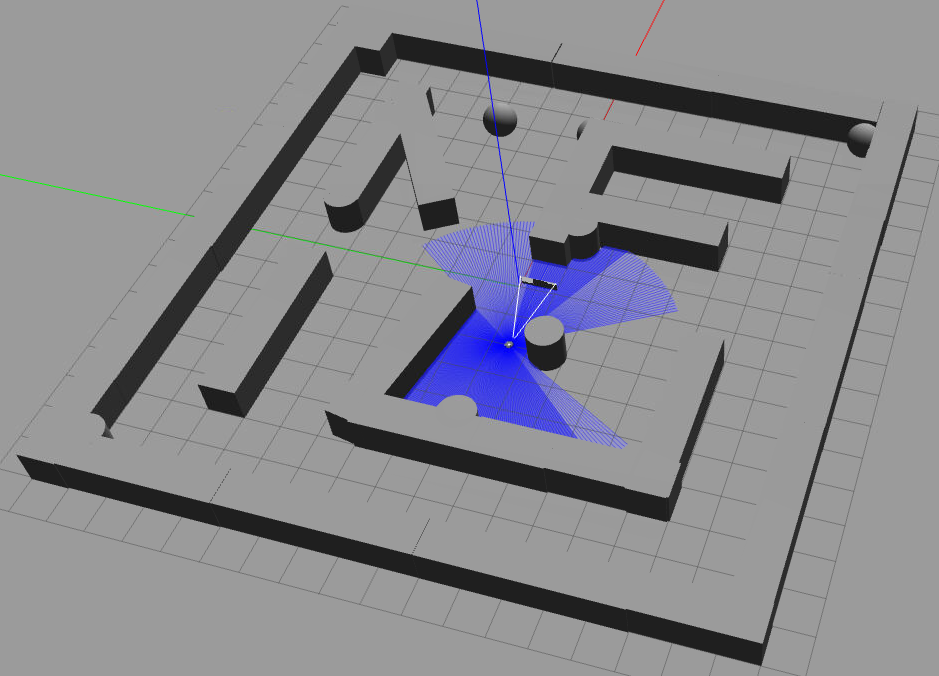
\includegraphics[height=11cm]{./images/mapa1.png}
    \caption{Widok mapy w rzucie izometrycznym}
\end{figure}


\begin{figure}[!htb]
    \centering
    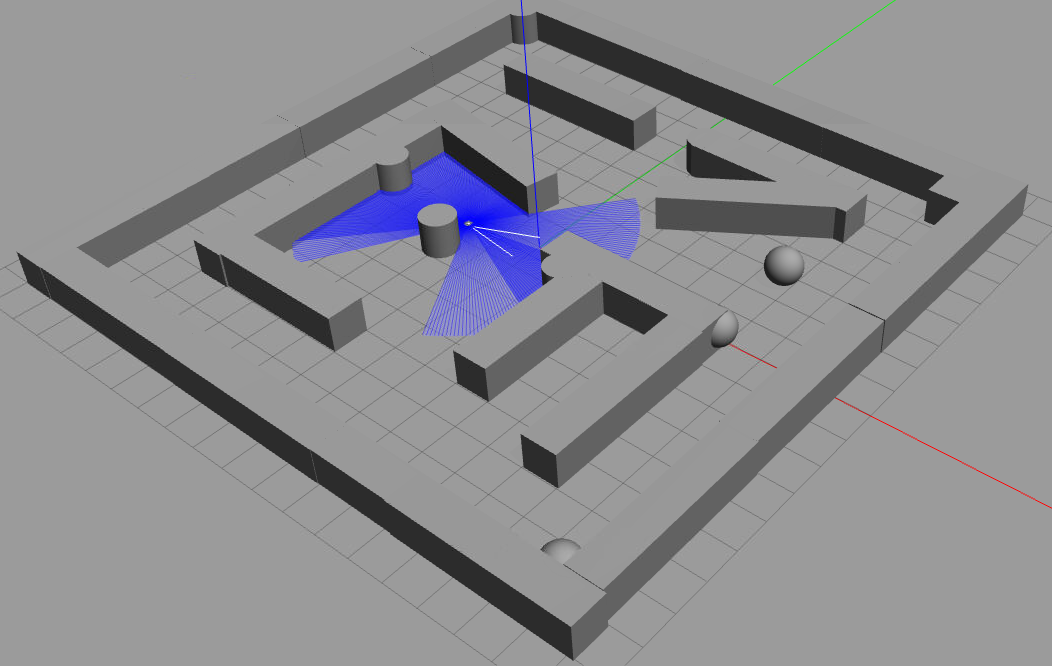
\includegraphics[height=9.5cm]{./images/mapa2.png}
    \caption{Inny rzut izometryczny}
\end{figure}


\begin{figure}[!htb]
    \centering
    
\includegraphics[height=9.5cm]{./images/rviz.png}
    \caption{Model mapy do nawigacji w Rvizz}
\end{figure}



\clearpage\newpage
\section{Kod}

\subsection{Zasada działania}

\vsp 
Nasz system składa się z dwóch programów, które można zaklasyfikować jako back-end i front-end. Pierwszy program komunikuje się bezpośrednio w robotem, a drugi program komunikuje się z użytkownikiem końcowym. Oba programy wymieniają się informacjami za pomocą wspólnej bazy danych w technologii ``sqlite3''. 

\vsp
\subsubsection*{Baza danych}

\noindent Baza danych zawiera jedną tabele, której definicja w naszym narzędziu ORM jest poniżej. Każdy rekord w tabeli \texttt{schedules} odpowiada jednemu rozkazowi, który ma zostać wydany robotowi.

\vsp\vsp

\begin{lstlisting}

self.tables = {
    "schedules":
        BaseTable(name="schedules", fields=[
            IntegerFieldSQLite(name="id", primary_key=True),
            BoolFieldSQLite(name="is_completed", null=False, default=0),
            BoolFieldSQLite(name="in_progress", null=False, default=0),
            BoolFieldSQLite(name="timestamp", null=False),
            IntegerFieldSQLite(name="x", null=False),
            IntegerFieldSQLite(name="y", null=False),
            IntegerFieldSQLite(name="z", null=False),
        ]),
}

\end{lstlisting}

\vsp
\vsp

\noindent Odczytywanie następnego polecenia odpowiada się za pomocą kwerendy

\vsp 

\begin{lstlisting}[language=SQL]
SELECT * FROM schedules WHERE is_completed=0 AND in_progress=0 ORDER BY timestamp
\end{lstlisting}



\newpage
\subsubsection*{Back-end}

Wydawanie rozkazów typu \texttt{navigate\_to\_pose} zaimplementowaliśmy za pomocą timera, który co jedną sekundę wykonuje zapytanie do bazy danych. Baza danych odpowiada listą zadań, które robot ma wykonać, a program decyduje, które zadanie mu przydzielić. Po wykonaniu zadania robot zgłasza koniec akcji, co w programie powoduje wykonanie kodu, który dokonuje odpowiednich zmian w bazie danych.

\vsp

\begin{lstlisting}

class Taxi(Node):
def __init__(self): 
    super().__init__('taxi')

    self.is_robot_busy = False
    
    self.publisher_ = self.create_publisher(Twist, 
                                            'cmd_vel',
                                            10)
    


    self.timer = self.create_timer(
        1.0,
        self.read_db)

[...]

def read_db(self):
    navigate_action = ActionClient(
        taxi, 
        NavigateToPose,
        '/navigate_to_pose')


    BASE_DIR = Path("/home/ubuntu/turtlebot3_ws/src/jupyter_notebooks")
    storage_obj = BaseStorage(BASE_DIR)
    with storage_obj as s:
        cursor = s.conn.cursor()
        rows = cursor.execute("SELECT * FROM schedules WHERE is_completed=0 AND in_progress=0 ORDER BY timestamp").fetchall()


    if len(rows) > 0 and not self.is_robot_busy:
        navigate_pose_goal = NavigateToPose.Goal()    
        goal_pose = PoseStamped()
        goal_pose.header.stamp = self.get_clock().now().to_msg()
        goal_pose.pose.position.x = float(rows[0]["x"])
        goal_pose.pose.position.y = float(rows[0]["y"])
        goal_pose.pose.orientation.z = 0.0
        goal_pose.pose.orientation.w = 0.0
        navigate_pose_goal.pose = goal_pose

        self.goal_id = rows[0]["id"]

        goal_future_pose = navigate_action.send_goal_async(navigate_pose_goal, feedback_callback=self.print_feedback_goal)

        goal_future_pose.add_done_callback(self.received_task)


[...]

    def history_success(self, future):
    BASE_DIR = Path("/home/ubuntu/turtlebot3_ws/src/jupyter_notebooks")

    storage_obj = BaseStorage(BASE_DIR)
    with storage_obj as s:
        cursor = s.conn.cursor()
        rows = cursor.execute(f"UPDATE schedules SET is_completed=1, in_progress=0 WHERE id={self.goal_id}")
        s.conn.commit()

    self.is_robot_busy = False
    
\end{lstlisting}




\newpage
\subsubsection*{Front-end}

Aplikacja front-end pozwala użytkownikowi komunikować się z robotem. Aplikacja opiera się na interaktywnych komórkach Jupyter Notebook, w których użytkownik musi wpisać miejsce do, którego robot ma się udać. W rzeczywistosci mogłoby to wyglądać w następujący sposób. Użytkownik w aplikacji mobilnej wpisuje, gdzie się aktualnie znajduje, robot do niego przyjeżdża. Następnie po wejściu do taksówki użytkownik wpisuje w aplikacji dokąd chcę jechać, a robot taxi go tam zabiera.

\vsp\vsp

\begin{lstlisting}
def send_robot(x="0", y="0"):
    BASE_DIR = Path("/home/ubuntu/turtlebot3_ws/src/jupyter_notebooks")

    timestamp = int(time.time()*1000)

    storage_obj = BaseStorage(BASE_DIR)
    with storage_obj as s:
        timestamp = int(time.time()*1000)
        s.insert_row({"is_completed":False, "in_progress":False, "x":float(x), "y":float(y), "z":0, "timestamp": timestamp}, "schedules")
    
\end{lstlisting}
    
\vsp\vsp

\begin{figure}[!htb]
    \centering
    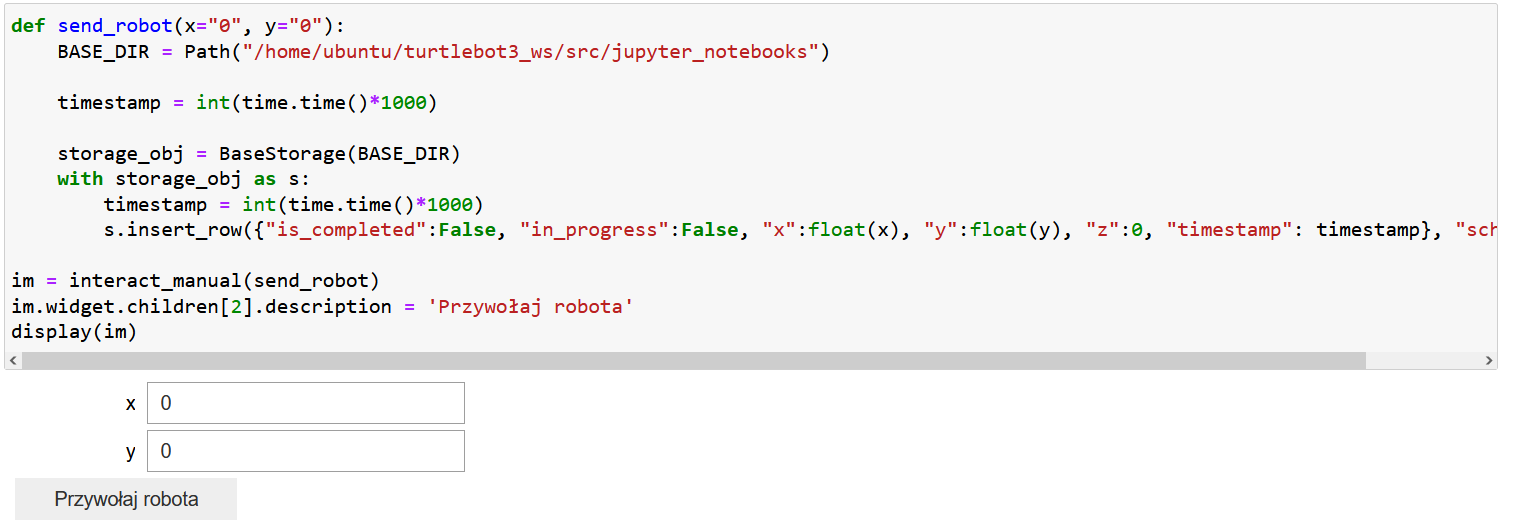
\includegraphics[width=18cm]{./images/interact.png}
    \caption{Interfejs użytkownika}
\end{figure}


\end{document}